\documentclass{article}
\usepackage{listings}
\usepackage{mathrsfs}
\usepackage[utf8]{inputenc}
\usepackage{amssymb}
\usepackage{lipsum}
\usepackage{amsmath}
\usepackage{fancyhdr}
\usepackage{geometry}
\usepackage{scrextend}
\usepackage[english,german]{babel}
\usepackage{titling}
\setlength{\droptitle}{-3cm}
\usepackage{tikz}
\usepackage{algorithm,algpseudocode}
\usepackage[doublespacing]{setspace}
\usetikzlibrary{datavisualization}
\usetikzlibrary{datavisualization.formats.functions}
\usepackage{polynom}
\usepackage{amsmath}
\usepackage{verbatim}
\usepackage{gauss}
\usepackage{tkz-euclide}
\usetikzlibrary{datavisualization}
\usetikzlibrary{datavisualization.formats.functions}
\author{
Alexander Mattick Kennung: qi69dube\\
Kapitel 1
}
\usepackage{import}
\date{\today}
\geometry{a4paper, margin=2cm}
\usepackage{stackengine}
\parskip 1em
\newcommand\stackequal[2]{%
  \mathrel{\stackunder[2pt]{\stackon[4pt]{=}{$\scriptscriptstyle#1$}}{%
  $\scriptscriptstyle#2$}}
 }
\makeatletter
\renewcommand*\env@matrix[1][*\c@MaxMatrixCols c]{%
  \hskip -\arraycolsep
  \let\@ifnextchar\new@ifnextchar
  \array{#1}}
\makeatother
\lstset{
  language=haskell,
}
\lstnewenvironment{code}{\lstset{language=Haskell,basicstyle=\small}}{}
\usepackage{enumitem}
\setlist{nosep}
\usepackage{titlesec}

\titlespacing*{\subsection}{0pt}{2pt}{3pt}
\titlespacing*{\section}{0pt}{0pt}{5pt}
\titlespacing*{\subsubsection}{0pt}{1pt}{2pt}
\title{Vorlesung 4}


\begin{document}
	\maketitle
	\section{Hausaufgabe 28}
	a)\\
	\[f(x)=\begin{cases}0&x<a\lor x>b\\\frac{4}{(b-a)^2}x-\frac{4a}{(b-a)^2}&a\leq x<\frac{a+b}{2}\\ \frac{-4}{(b-a)^2}x+\frac{4b}{(b-a)^2}&\frac{a+b}{2}\leq x\leq b\end{cases}\]
	Integral von $-\infty$ bis $\infty$ muss eins sein.\\
	\[\int f(x)dx = \int\begin{cases}0&x<a\lor x>b\\\frac{4}{(b-a)^2}x-\frac{4a}{(b-a)^2}&a\leq x<\frac{a+b}{2}\\ \frac{-4}{(b-a)^2}x+\frac{4b}{(b-a)^2}&\frac{a+b}{2}\leq x\leq b\end{cases} dx = \begin{cases}0&x<a\lor x>b\\\frac{2}{(b-a)^2}x^2-\frac{4ax}{(b-a)^2}&a\leq x<\frac{a+b}{2}\\ \frac{-2}{(b-a)^2}x^2+\frac{4bx}{(b-a)^2}&\frac{a+b}{2}\leq x\leq b\end{cases}\]
	Relevant für den integral ist nur der nicht-null Bereich: zuerst der zweite Fall\\
	$$(\lim\limits_{x\to\frac{a+b}{2}}\frac{2x^2}{(b-a)^2}-\frac{4ax}{(b-a)^2})-(\frac{2a^2}{(b-a)^2}-\frac{4a^2}{(b-a)^2})$$
	$$(\lim\limits_{x\to\frac{a+b}{2}}\frac{2x^2}{(b-a)^2}-\frac{4ax}{(b-a)^2})+\frac{2a^2}{(b-a)^2}$$
	$$(\frac{2(\frac{a+b}{2})^2}{(b-a)^2}-\frac{4a(\frac{a+b}{2})}{(b-a)^2})+\frac{2a^2}{(b-a)^2}$$
	$$\frac{\frac{1}{2}(a+b)(b-3a)}{(b-a)^2}+\frac{2a^2}{(b-a)^2}$$
	$$\frac{\frac{1}{2}(a+b)(b-3a)+2a^2}{(b-a)^2}$$
	$$\frac{\frac{1}{2}(a+b)(b-3a)+2a^2}{(b-a)^2}$$
	$$\frac{\frac{1}{2}(a-b)^2}{(b-a)^2}=\frac{1}{2}$$
	Jetzt der dritte Fall:\\
	Hier jetzt zuerst zusammenfassen $\frac{-2}{(b-a)^2}x^2+\frac{4bx}{(b-a)^2}= \frac{2x(2b-x)}{(b-a)^2}$\\
	$$\frac{2b(2b-b)}{(b-a)^2}-\frac{2\frac{a+b}{2}(2b-\frac{a+b}{2})}{(b-a)^2}$$
	$$\frac{2b(b)-(a+b)(2b-\frac{a+b}{2})}{(b-a)^2}$$
	$$\frac{2b^2-(2ba-\frac{a+b}{2}a+2b^2-\frac{a+b}{2}b)}{(b-a)^2}$$
	$$\frac{2b^2-2ba+\frac{a+b}{2}a-2b^2+\frac{a+b}{2}b}{(b-a)^2}$$
	$$\frac{-2ba+\frac{a+b}{2}a+\frac{a+b}{2}b}{(b-a)^2}$$
	$$\frac{\frac{1}{2}(a-b)^2}{(b-a)^2}=\frac{1}{2}$$
	Die Summe von Fall 2 und 3 ist also:\\
	$\frac{1}{2}+\frac{1}{2}=1$\\
	Somit ist $f$ eine Wahrscheinlichkeitsdichtefunktion\\
	\\
	\\
	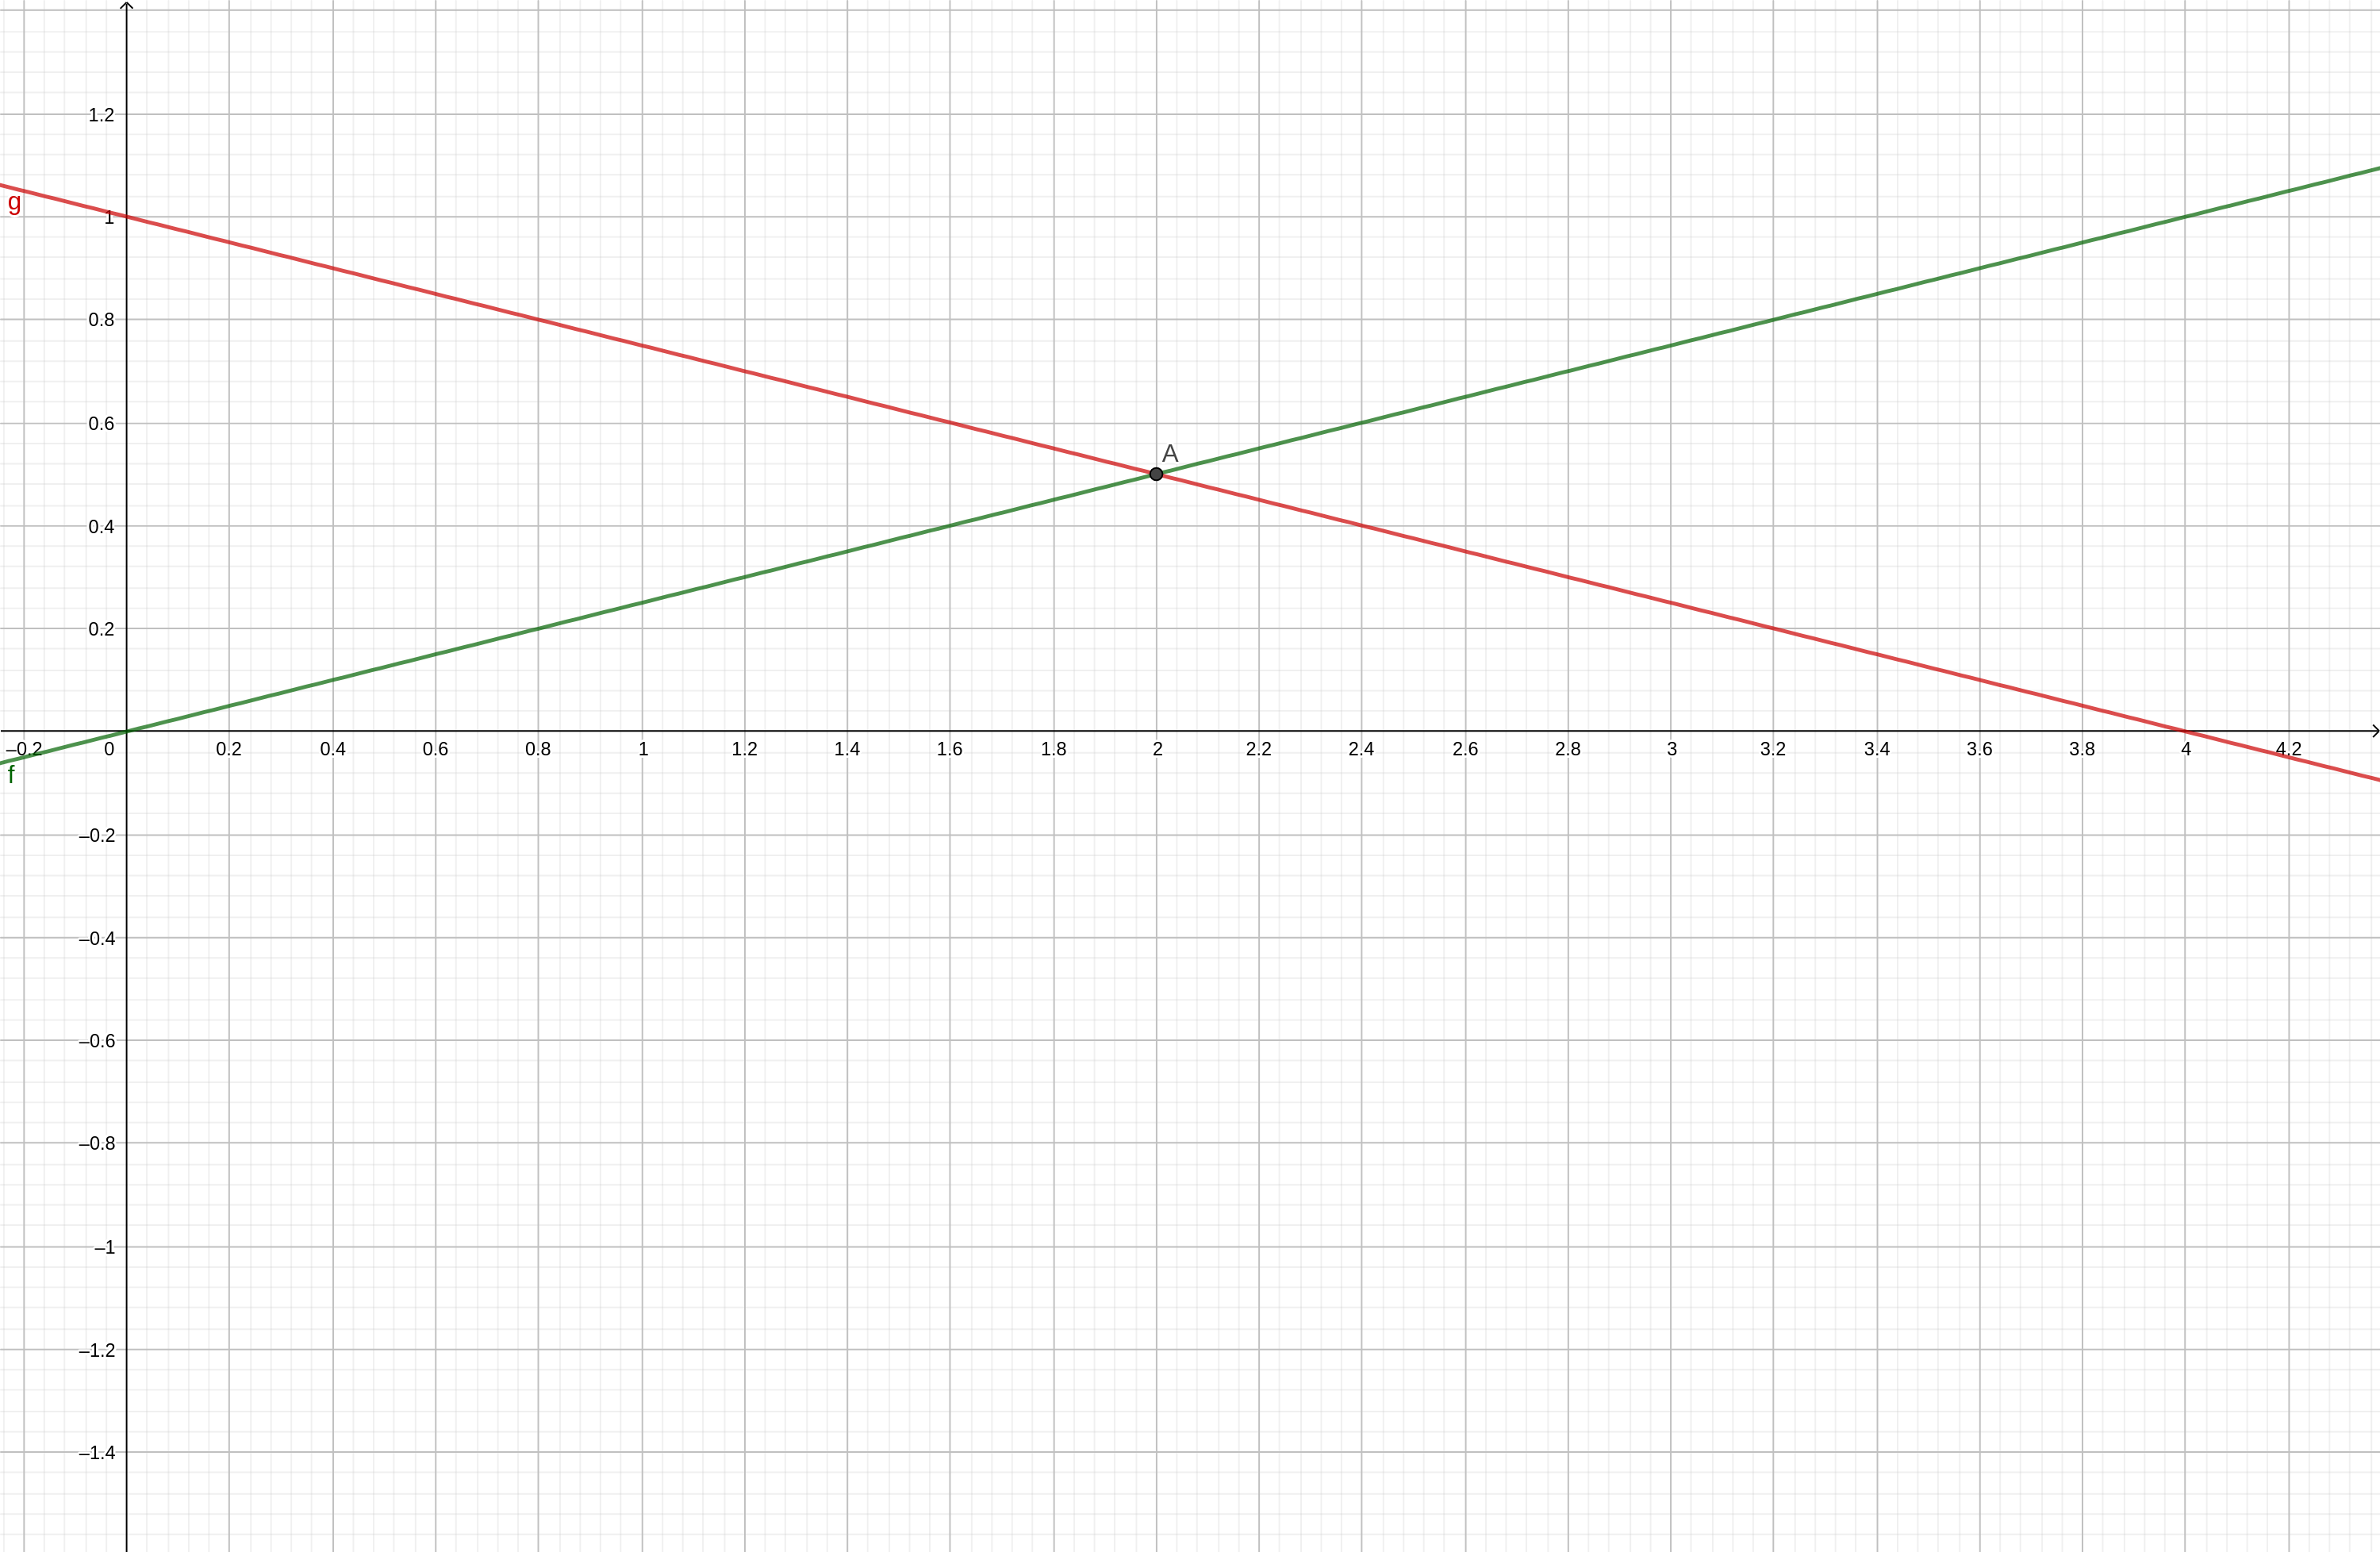
\includegraphics[width=256px]{geogebra-export.png}\\
	TODO: ZEICHNEN!\\
	b) Wir haben jetzt das Integral, also kann einfach $F(0.25a+0.75b)-F(0.75a+0.25b)$\\
	Da $a<b$ ist, kann man $0.25a+0.75b>0.25a+0.75a>a$ und $0.75a+0.25b>0.75a+0.25a>a$ schließen. (Nie Fall 1)\\
	Weiterhin gilt $0.75a+0.25b=\frac{1}{4} (3a+b)<\frac{a+b}{2}\iff (3a+b)<\frac{4(a+b)}{2}\iff(3a+b)<2a+2b\iff a+b<2b\iff a<b$ ist immer Wahr (nach definition). Also landen wir in Fall 2.\\
	Weiterhin gilt $0.25a+0.75b = \frac{1}{4} (a+3b)> \frac{a+b}{2}\iff (a+3b)> 2(a+b)\iff a+b>2a\iff b>a$ (per definition wahr) Also hier Fall 3:\\
	Wir nutzen die Symmetrie von f um $\frac{a+b}{2}$ aus.\\
	Dies gilt, da zwischen a und b bis genau $\frac{a+b}{2}$ gestiegen wird, und dann mit der gleichen (negativen) Steigung wieder fällt. Außerdem gilt, dass die funktion in $\frac{a+b}{2}$ für beide Fälle den gleichen Wert besitzt.\\
	Somit lässt sich vereinfachen:\\
	$[\lim\limits_{x\to \frac{a+b}{2}} F_2(x)-F_2(0.75a+0.25b)]+ [F_3(0.25a+0.75b)-F_3(\frac{a+b}{2})]$\\
	Dies liefert:\\
	$[\frac{2}{(b-a)^2}(\frac{a+b}{2})^2-\frac{4a(\frac{a+b}{2})}{(b-a)^2}-(\frac{2}{(b-a)^2}(0.75a+0.25b)^2-\frac{4a(0.75a+0.25b)}{(b-a)^2})]+ [\frac{-2}{(b-a)^2}(0.25a+0.75b)^2+\frac{4b(0.25a+0.75b)}{(b-a)^2}-(\frac{-2}{(b-a)^2}(\frac{a+b}{2})^2+\frac{4b(\frac{a+b}{2})}{(b-a)^2})]$\\
	Zusammenfassen:\\
	$[\frac{2}{(b-a)^2}(\frac{a+b}{2})^2-\frac{4a(\frac{a+b}{2})}{(b-a)^2}-\frac{2}{(b-a)^2}(0.75a+0.25b)^2+\frac{4a(0.75a+0.25b)}{(b-a)^2}]+ [\frac{-2}{(b-a)^2}(0.25a+0.75b)^2+\frac{4b(0.25a+0.75b)}{(b-a)^2}-\frac{-2}{(b-a)^2}(\frac{a+b}{2})^2-\frac{4b(\frac{a+b}{2})}{(b-a)^2}]$\\
	$[\frac{4}{(b-a)^2}(\frac{a+b}{2})^2-\frac{4(a+b)(\frac{a+b}{2})}{(b-a)^2}-\frac{2}{(b-a)^2}(0.75a+0.25b)^2+\frac{4a(0.75a+0.25b)}{(b-a)^2}]+ [\frac{-2}{(b-a)^2}(0.25a+0.75b)^2+\frac{4b(0.25a+0.75b)}{(b-a)^2}]$\\
	$$\frac{4(\frac{a+b}{2})^2-4(a+b)(\frac{a+b}{2})-2(0.75a+0.25b)^2+4a(0.75a+0.25b)-2(0.25a+0.75b)^2+4b(0.25a+0.75b)}{(b-a)^2}$$\\
	$$\frac{4(\frac{a+b}{2})(\frac{a+b}{2}-(a+b))-2(0.75a+0.25b)^2+3a^2+1ba-2(0.25a+0.75b)^2+(1ba+3b^2)}{(b-a)^2}$$\\
	$$\frac{4(\frac{a+b}{2})(\frac{a+b}{2}-(a+b))+3a^2+2ba-1.25a^2-1.5ab-1.25b^2+ 3b^2}{(b-a)^2}$$
	$$\frac{-(a+b)^2+3a^2+2ba-1.25a^2-1.5ab-1.25b^2+ 3b^2}{(b-a)^2}$$
	$$\frac{-(a^2+2ab+b^2)+3a^2+2ba-1.25a^2-1.5ab-1.25b^2+ 3b^2}{(b-a)^2}$$
	$$\frac{-a^2-2ab-b^2+3a^2+2ba-1.25a^2-1.5ab-1.25b^2+ 3b^2}{(b-a)^2}$$
	$$\frac{2a^2-1.25a^2-1.5ab-1.25b^2+ 2b^2}{(b-a)^2}$$
	$$\frac{0.75a^2-1.5ab+0.75b^2}{(b-a)^2}$$
	$$\frac{0.75(a^2-2ab+b^2)}{(b-a)^2}$$
	$$\frac{0.75(b-a)^2}{(b-a)^2}=0.75$$


	Im fall von $a=0$ und $b=4$
	$$\frac{2*2^2}{4^2}-\frac{2*1^2}{4^2}+\frac{-2*3^2}{4^2}+\frac{4*4*3}{4^2} -(\frac{-2*2^2}{4^2}+\frac{4*2*2}{4^2})$$
	$$\frac{1}{2}-\frac{1}{8}-\frac{9}{8}+3+\frac{1}{2}-2 =\frac{3}{4}$$
	\section{Hausaufgabe 29}
	a) $F(x)=\begin{cases}0&x\leq 0\\
	\ln(1+\sin x)& 0<x\leq\frac{3\pi}{4}\\
	1 &x>\frac{3\pi}{4}
	\end{cases}$
	Das der $\lim\limits_{x\to\infty}=1$ und $\lim\limits_{x\to-\infty}=0$ ist offensichtlich.\\
	Zuerst die Funktion ableiten: $f(x)=\begin{cases}0&x\leq 0\\
	\frac{\cos x}{1+\sin x}& 0<x\leq\frac{3\pi}{4}\\
	0 &x>\frac{3\pi}{4}
	\end{cases}$
	Der zweite Fall $f_2(x)=\frac{\cos x}{1+\sin x}\stackequal{!}{}0\iff \cos x =0\iff x=\frac{1}{2}\in(0,\frac{3}{4}\pi]$ also ist $F(x)$ nicht monoton steigend, also keine Verteilungsfunktion.\\
	b) $F(x)=(1-exp(-x))1_{[0,\infty)}(x)$
	Man muss nur $x\geq0$ betrachten, da sonst $1_{[0,\infty)}(x)=0$ ist. In diesem Fall spielt $1_{[0,\infty)}(x)$ keine Rolle beim Wert.\\
	$f(x) = exp(-x)$ für $x\geq 0$\\
	$f(x)\neq 0$ für alle x, also ist die funktion isoton.\\
	Im limes wird $\lim\limits_{x\to\infty} F(x)=\lim\limits_{x\to\infty} (1-exp(-x))1_{[0,\infty)}(x) = 1$, bzw null für $\lim\limits_{x\to-\infty} F(x)=\lim\limits_{x\to-\infty} (1-exp(-x))1_{[0,\infty)}(x)=0$ Wegen der $1_{[0,\infty)}(x)$ funktion.\\
	Für positive/negative Werte ist $F(x)$ stetig, also insbesondere rechtsseitig stetig.\\
	Nur in Null könnte F nicht stetig sein. Es gilt jedoch:\\
	$\lim\limits{x\to0^-} F(x) = (1-exp(-x))1_{[0,\infty)}(x)=0 $ Wegen sprungfunktion.\\
	und $\lim\limits{x\to0^+} F(x) = (1-exp(-x))1_{[0,\infty)}(x)=0 $ Wegen $\lim\limits{x\to0^+}(1-exp(-x))=0$.\\
	Somit ist F stetig.\\
	F ist also eine Verteilungsfunktion.\\
\end{document}